\chapter{Теория}
\label{ch:theory}

    \section{Термины и определения}
    В настоящей итоговой аттестационной работе применяют следующие термины с соответствующими определениями:
    
    Интеллектуальные технические системы: Системы, основанные на применении искусственного интеллекта, машинного обучения и других технологий для выполнения сложных задач, требующих анализа, обработки и принятия решений.
    
    Машинное обучение: Область искусственного интеллекта, которая изучает методы и алгоритмы, позволяющие компьютерам самостоятельно извлекать знания из данных и обучаться на основе опыта.
    
    Искусственный интеллект: Наука и технология, занимающаяся созданием компьютерных систем, способных выполнять задачи, требующие интеллектуальных способностей человека, таких как распознавание образов, обработка языка и принятие решений.
    
    Компьютерное зрение: Область искусственного интеллекта, изучающая методы и алгоритмы анализа и интерпретации изображений и видео с помощью компьютеров.
    
    Робототехника: Наука и технология, изучающая проектирование, разработку и управление роботами, основанными на принципах и методах инженерии искусственного интеллекта.
    
    Автоматизированные системы: Системы, в которых задачи и операции выполняются автоматически без участия человека, используя компьютерные технологии и интеллектуальные алгоритмы.
    
    Нейронные сети: Математическая модель, вдохновленная работой нервной системы, состоящая из соединенных и взаимодействующих искусственных нейронов, используемая для обработки информации и выполнения задач машинного обучения.
    
    Глубокое обучение: Метод машинного обучения, основанный на использовании искусственных нейронных сетей с большим количеством скрытых слоев для извлечения иерархических представлений и обучения сложным задачам.
    
    Экспертные системы: Интеллектуальные компьютерные системы, способные имитировать знания и экспертизу человека в определенной области для принятия решений или решения сложных проблем.
    
    Кластерный анализ: Метод анализа данных, направленный на группировку объектов в пределах одного кластера на основе их сходства или близости.
    
    Обработка естественного языка: Область искусственного интеллекта, изучающая методы анализа, понимания и генерации естественного языка, используемого людьми, для различных задач, включая машинный перевод и автоматическую обработку текста.
    
    Автономные системы: Системы, способные функционировать и принимать решения без постоянного участия человека, обладающие возможностью адаптироваться к изменяющимся условиям и окружающей среде.
    
    Обучение с подкреплением: Метод машинного обучения, в котором агент самостоятельно осуществляет принятие решений и обучается на основе награды или штрафа, получаемых в процессе взаимодействия с окружающей средой.
    
    Большие данные: Массивы данных огромного объема и сложности, которые требуют специальных методов и инструментов для их хранения, анализа и использования.
    
    Алгоритмы генетического программирования: Метод оптимизации искусственного интеллекта, вдохновленный принципами естественного отбора и генетики, использующий эволюционные процессы для создания программного кода или моделей.
    
    Самообучение: Способность системы или алгоритма к самостоятельному извлечению и обновлению знаний на основе накопленного опыта и данных без явного вмешательства программиста или оператора.
    
    Анализ данных: Процесс извлечения, очистки, преобразования и моделирования данных с целью выявления закономерностей, тенденций и информации, полезной для принятия решений и планирования.
    
    Разведочный анализ данных: Метод анализа данных, направленный на исследование данных для выявления новых паттернов, связей и трендов, неизвестных ранее.
    
    Виртуальные агенты: Интеллектуальные компьютерные агенты, которые имитируют поведение и взаимодействие людей, обладая способностью обрабатывать естественный язык, распознавать речь и выполнять задачи в виртуальной среде.
    
    Автоматизированное принятие решений: Процесс, в ходе которого система или алгоритм принимает определенное решение или рекомендацию на основе анализа данных, логики и предопределенных правил.
    
    Интеллектуальные алгоритмы: Алгоритмы, использующие искусственный интеллект и машинное обучение для выполнения сложных задач, требующих анализа, классификации, оптимизации и прогнозирования.
    
    Облачные вычисления: Модель предоставления компьютерных ресурсов, таких как вычислительная мощность, хранение данных и программное обеспечение, через интернет с использованием удаленных серверов и сетевых сервисов.
    
    Анализ рисков: Процесс и методы оценки потенциальных угроз, возможных неблагоприятных событий и их вероятности, связанных с использованием интеллектуальных технических систем, а также разработка стратегий и мер по снижению рисков.
    
    Компьютерная симуляция: Метод моделирования и воссоздания реальных или вымышленных процессов, систем и ситуаций с использованием компьютерных моделей, что позволяет проводить различные эксперименты и исследования без реального исполнения.
    
    \section{Непосредственно теория}
    Роль и пути развития информационных технологий в современных условиях

    Роль развития информационных технологий в области интеллектуальных технических систем заключается в создании и совершенствовании инструментов, методов и алгоритмов, позволяющих разрабатывать и эффективно использовать такие системы. Информационные технологии играют ключевую роль в развитии Интеллектуальных технических систем, обеспечивая их функционирование, анализ данных, обработку информации и принятие решений.

    Ниже приведены основные роли развития информационных технологий в области интеллектуальных технических систем:
    \begin{enumerate}
        \item Обеспечение вычислительной мощности: Развитие информационных технологий, таких как высокопроизводительные вычисления, параллельные вычисления и облачные вычисления, обеспечивает достаточную вычислительную мощность для работы сложных Интеллектуальных технических систем;
        \item Разработка алгоритмов и моделей: Информационные технологии позволяют разрабатывать и улучшать алгоритмы и модели, используемые в Интеллектуальных технических системах. Это включает в себя разработку методов машинного обучения, нейронных сетей, алгоритмов обработки естественного языка и других методов искусственного интеллекта;
        \item Сбор и анализ данных: Развитие информационных технологий способствует сбору и хранению больших объемов данных, необходимых для обучения и функционирования Интеллектуальных технических систем. Технологии обработки данных и анализа больших данных позволяют извлекать ценные знания из накопленных данных;
        \item Развитие интерфейсов и взаимодействия: Информационные технологии способствуют разработке интуитивно понятных и эффективных пользовательских интерфейсов для Интеллектуальных технических систем. Это включает в себя разработку графических интерфейсов, голосовых интерфейсов, виртуальной и дополненной реальности;
        \item Обеспечение безопасности и конфиденциальности: Развитие информационных технологий также направлено на обеспечение безопасности и конфиденциальности данных в Интеллектуальных технических системах. Разработка криптографических методов, аутентификации пользователей и защиты данных является важной составляющей развития ИТ в этой области;
        \item Интеграция и оптимизация систем: Информационные технологии играют важную роль в интеграции различных компонентов Интеллектуальных технических систем и их оптимизации. Развитие технологий интеграции, стандартов обмена данных и оптимизации алгоритмов способствует более эффективному и совместному функционированию системы.
        Развитие информационных технологий в области интеллектуальных технических систем является ключевым фактором для их успешного развития и применения в различных областях, таких как автоматизация производства, медицина, транспорт, энергетика и другие.
        \item Автоматизация процессов: Информационные технологии позволяют автоматизировать различные процессы в Интеллектуальных технических системах. Это включает в себя автоматическую обработку данных, принятие решений на основе алгоритмов и моделей, автоматическое управление системами и т.д. Автоматизация процессов снижает ручной труд, повышает эффективность и точность работы систем;
        \item Разработка умных алгоритмов и систем: Информационные технологии играют важную роль в разработке умных алгоритмов и систем, которые способны самостоятельно обучаться, принимать решения и адаптироваться к изменяющейся среде. Это включает в себя разработку алгоритмов машинного обучения, нейронных сетей, генетических алгоритмов и других интеллектуальных методов;
        \item Оптимизация ресурсов: Развитие информационных технологий позволяет оптимизировать использование ресурсов в Интеллектуальных технических системах. Это включает в себя оптимизацию вычислительных ресурсов, энергопотребления, использования сенсоров и других компонентов системы. Оптимизация ресурсов способствует повышению эффективности и экономии затрат;
        \item Интеллектуальная аналитика: Информационные технологии позволяют проводить анализ данных и извлекать ценную информацию из больших объемов данных в Интеллектуальных технических системах. Это включает в себя методы обработки и анализа данных, визуализацию данных, статистический анализ и прогнозирование. Интеллектуальная аналитика помогает принимать обоснованные решения и выявлять скрытые закономерности в данных.
    \end{enumerate}

    Развитие информационных технологий в области вычислительной мощности играет решающую роль в обеспечении эффективной работы сложных интеллектуальных технических систем. Вот несколько ключевых аспектов, связанных с обеспечением вычислительной мощности:
    \begin{enumerate}
        \item Высокопроизводительные вычисления: Развитие информационных технологий способствует созданию и совершенствованию высокопроизводительных вычислительных систем. Это включает разработку мощных процессоров, графических ускорителей, специализированных вычислительных устройств и кластерных систем. Высокопроизводительные вычисления позволяют обрабатывать большие объемы данных и выполнять сложные вычислительные задачи;
        \item Параллельные вычисления: Информационные технологии также способствуют развитию методов и алгоритмов параллельных вычислений. Параллельные вычисления позволяют выполнять несколько вычислительных задач одновременно, разделяя их на более мелкие подзадачи, которые выполняются параллельно на разных вычислительных ресурсах. Это увеличивает скорость выполнения задач и обеспечивает более эффективное использование вычислительных ресурсов;
        \item Облачные вычисления: Развитие информационных технологий привело к появлению облачных вычислений, которые предоставляют доступ к вычислительным ресурсам через интернет. Облачные вычисления позволяют Интеллектуальным техническим системам получать вычислительную мощность по требованию, масштабировать свои вычисления в зависимости от нагрузки и управлять ресурсами более гибко. Это позволяет снизить затраты на оборудование и обеспечить гибкость в работе системы;
        \item Квантовые вычисления: Одним из перспективных направлений развития информационных технологий являются квантовые вычисления. Квантовые компьютеры используют квантовые явления, такие как суперпозиция и квантовая интерференция, для выполнения вычислений. Квантовые вычисления обладают потенциалом решать задачи, которые недоступны для классических компьютеров. Развитие квантовых вычислений может значительно усилить вычислительную мощность Интеллектуальных технических систем и открыть новые возможности в решении сложных задач.
    \end{enumerate}

    Обеспечение вычислительной мощности является критическим аспектом развития Интеллектуальных технических систем. Развитие информационных технологий в этой области позволяет создавать более мощные, эффективные и гибкие системы, способные решать сложные задачи и принимать интеллектуальные решения.

    Разработка алгоритмов и моделей является ключевым аспектом в области Интеллектуальных технических систем. Информационные технологии играют важную роль в этом процессе, обеспечивая разработку и улучшение различных типов алгоритмов и моделей. Вот несколько важных аспектов разработки алгоритмов и моделей:
    \begin{enumerate}
        \item Машинное обучение: Информационные технологии позволяют разрабатывать алгоритмы машинного обучения, которые позволяют системам извлекать информацию и обучаться на основе данных. Машинное обучение включает в себя методы, такие как классификация, регрессия, кластеризация и обучение с подкреплением. Развитие информационных технологий способствует созданию более эффективных и точных моделей машинного обучения;
        \item Нейронные сети: Информационные технологии также включают разработку и применение нейронных сетей, которые являются основой для многих Интеллектуальных технических систем. Нейронные сети моделируют работу нервной системы и позволяют системам обрабатывать сложные данные и распознавать образы. Развитие информационных технологий в области нейронных сетей приводит к созданию более глубоких и мощных моделей, способных обучаться на больших объемах данных;
        \item Алгоритмы обработки естественного языка: Информационные технологии развиваются и в области алгоритмов обработки естественного языка. Это позволяет системам понимать и обрабатывать человеческий язык, что открывает возможности для создания чат—ботов, систем автоматического перевода, анализа текстов и других приложений, связанных с языковой обработкой;
        \item Интеграция с большими объемами данных: Развитие информационных технологий позволяет эффективно работать с большими объемами данных, которые часто используются в Интеллектуальных технических системах. Разработка алгоритмов и моделей, способных обрабатывать и анализировать огромные массивы данных, является важным направлением развития.
    \end{enumerate}

    Развитие информационных технологий в области разработки алгоритмов и моделей открывает новые горизонты для Интеллектуальных технических систем. Они становятся более интеллектуальными, адаптивными и способными принимать сложные решения на основе данных. Это позволяет повысить эффективность и точность работы таких систем в различных сферах применения.

    Сбор и анализ данных являются неотъемлемой частью развития Интеллектуальных технических систем. Развитие информационных технологий играет ключевую роль в эффективном сборе, хранении и анализе больших объемов данных. Вот несколько важных аспектов, связанных с сбором и анализом данных:
    \begin{enumerate}
        \item Сенсоры и датчики: Развитие информационных технологий позволяет создавать и использовать различные типы сенсоров и датчиков для сбора данных. Например, в Интеллектуальных технических системах могут использоваться датчики с измерителями температуры, давления, влажности, а также различные виды камер и микрофонов для сбора аудио— и видеоданных. Развитие информационных технологий в этой области способствует созданию более точных и эффективных сенсорных систем;
        \item Большие данные: Развитие информационных технологий привело к росту объемов данных, накапливающихся в различных областях. Технологии хранения данных и обработки больших данных (Big Data) позволяют эффективно управлять и анализировать эти объемы информации. Интеллектуальные технические системы используют методы и алгоритмы обработки больших данных для извлечения ценных знаний и паттернов, что позволяет принимать более точные и обоснованные решения;
        \item Алгоритмы анализа данных: Развитие информационных технологий в области анализа данных способствует разработке эффективных алгоритмов для обработки и интерпретации собранных данных. Это включает методы машинного обучения, статистический анализ, анализ временных рядов, обработку естественного языка и другие подходы. Развитие алгоритмов анализа данных позволяет Интеллектуальным техническим системам обнаруживать закономерности, прогнозировать тренды, классифицировать данные и принимать основанные на данных решения.
    \end{enumerate}

    Развитие информационных технологий в области сбора и анализа данных является критическим фaktором в развитии Интеллектуальных технических систем. Оно обеспечивает доступ к большим объемам данных, а также инструменты и методы для их анализа и интерпретации. Это открывает новые возможности для принятия более интеллектуальных и обоснованных решений на основе данных.

    Развитие интерфейсов и взаимодействия является важным аспектом в области Интеллектуальных технических систем. Информационные технологии играют ключевую роль в создании удобных и эффективных пользовательских интерфейсов, которые обеспечивают удобство взаимодействия между человеком и системой. Вот несколько аспектов, связанных с развитием интерфейсов и взаимодействия:
    \begin{enumerate}
        \item Графические интерфейсы: Информационные технологии позволяют разрабатывать графические интерфейсы, которые предоставляют визуальное представление данных и функциональности Интеллектуальных технических систем. Это включает элементы управления, кнопки, меню, диаграммы, графики и другие компоненты, которые помогают пользователям взаимодействовать с системой интуитивно и эффективно;
        \item Голосовые интерфейсы: Развитие информационных технологий приводит к созданию голосовых интерфейсов, которые позволяют пользователям взаимодействовать с Интеллектуальными техническими системами с помощью голосовых команд и разговоров. Технологии распознавания речи и синтеза речи обеспечивают возможность общения и контроля системы через голосовые команды, что повышает удобство и доступность использования;
        \item Виртуальная и дополненная реальность: Развитие информационных технологий также способствует разработке виртуальной и дополненной реальности, которые предоставляют новые способы взаимодействия с Интеллектуальными техническими системами. Виртуальная реальность позволяет пользователям погружаться в виртуальное окружение и взаимодействовать с системой в 3D—пространстве, а дополненная реальность дополняет реальный мир информацией и визуальными элементами с помощью устройств, таких как смарт—очки;
        \item Адаптивные интерфейсы: Информационные технологии также способствуют разработке адаптивных интерфейсов, которые могут приспосабливаться к индивидуальным предпочтениям и потребностям пользователей. Это включает возможность персонализации интерфейса, изменения размеров шрифтов, цветовой схемы, расположения элементов и других аспектов, чтобы обеспечить наилучшее пользовательское взаимодействие.
    \end{enumerate}

    Развитие интерфейсов и взаимодействия в Интеллектуальных технических системах позволяет создавать более удобные, эффективные и интуитивно понятные способы взаимодействия между человеком и системой. Это повышает уровень комфорта, удовлетворенности пользователей и обеспечивает более эффективное использование таких систем в различных областях применения.

    Обеспечение безопасности и конфиденциальности является одним из наиболее значимых аспектов развития информационных технологий в области Интеллектуальных технических систем. Вот некоторые ключевые аспекты в этой области:
    \begin{enumerate}
        \item Криптографические методы: Развитие информационных технологий приводит к разработке и совершенствованию криптографических методов и алгоритмов, которые обеспечивают защиту данных путем их шифрования и расшифрования. Это позволяет сохранять конфиденциальность информации и предотвращать несанкционированный доступ к данным;
        \item Аутентификация пользователей: Информационные технологии позволяют разрабатывать различные методы аутентификации пользователей, чтобы убедиться в их подлинности и предотвратить несанкционированный доступ к системе. Это может включать использование паролей, биометрических данных (отпечатков пальцев, распознавания лица и прочих), двухфакторной аутентификации и других методов, обеспечивающих безопасность доступа;
        \item Защита данных: Развитие информационных технологий направлено на разработку механизмов и методов защиты данных от угроз и несанкционированного доступа. Это включает использование шифрования данных, механизмов контроля доступа, систем мониторинга и обнаружения вторжений, а также разработку стратегий резервного копирования данных и восстановления после сбоев;
        \item Обеспечение безопасности в сети: Развитие информационных технологий также включает разработку сетевых механизмов и протоколов, которые обеспечивают безопасную передачу данных между Интеллектуальными техническими системами и их компонентами. Это включает защиту от сетевых атак, уязвимостей и несанкционированного доступа к сетевым ресурсам.
    \end{enumerate}

    Обеспечение безопасности и конфиденциальности данных в Интеллектуальных технических системах является неотъемлемой частью развития информационных технологий.

    Интеграция и оптимизация систем являются важными аспектами развития информационных технологий в области Интеллектуальных технических систем. Ниже представлены основные аспекты, связанные с интеграцией и оптимизацией систем:
    \begin{enumerate}
        \item Интеграция компонентов: Информационные технологии обеспечивают интеграцию различных компонентов Интеллектуальных технических систем, включая аппаратное обеспечение, программное обеспечение, сенсоры, исполнительные механизмы и другие элементы. Развитие технологий интерфейсов и протоколов позволяет эффективно связывать и синхронизировать работу различных компонентов системы;
        \item Стандартизация данных: Интеграция систем требует стандартизации обмена данных между компонентами системы. Развитие информационных технологий способствует разработке стандартов и протоколов, которые облегчают обмен информацией между различными системами и устройствами. Это позволяет эффективно использовать данные, передаваемые между компонентами системы, и обеспечивает их совместную работу;
        \item Оптимизация алгоритмов: Развитие информационных технологий способствует постоянному улучшению и оптимизации алгоритмов, используемых в Интеллектуальных технических системах. Это включает разработку более эффективных алгоритмов машинного обучения, оптимизацию процессов принятия решений, улучшение алгоритмов обработки данных и других методов, направленных на повышение производительности и функциональности системы;
        \item Оптимизация процессов: Информационные технологии также помогают оптимизировать процессы работы Интеллектуальных технических систем. Это включает автоматизацию и оптимизацию рабочих процессов, использование алгоритмов планирования и оптимизации, анализ данных для выявления узких мест и повышение эффективности системы в целом.
    \end{enumerate}

    Интеграция и оптимизация систем в Интеллектуальных технических системах позволяют достичь более эффективной и совместной работы компонентов системы, улучшить производительность и функциональность системы в целом. Это способствует более эффективному использованию ресурсов, повышению качества работы и улучшению пользовательского опыта.

    Принятие решений на основе алгоритмов и моделей: Информационные технологии позволяют разрабатывать и использовать алгоритмы и модели для автоматического принятия решений в Интеллектуальных технических системах. Это может включать использование методов машинного обучения, нейронных сетей, экспертных систем и других методов искусственного интеллекта для анализа данных и принятия оптимальных решений.
    
    Автоматизация процессов в Интеллектуальных технических системах приводит к повышению производительности, улучшению качества работы, снижению риска ошибок и увеличению общей эффективности системы. Это способствует достижению более оптимальных и результативных результатов в различных сферах, включая производство, транспорт, здравоохранение, энергетику и другие области применения Интеллектуальных технических систем.

    Оптимизация ресурсов является важным аспектом развития информационных технологий в области Интеллектуальных технических систем. Вот некоторые ключевые аспекты оптимизации ресурсов:
    \begin{enumerate}
        \item Оптимизация вычислительных ресурсов: Информационные технологии позволяют оптимизировать использование вычислительных ресурсов, таких как процессоры, память и хранилище данных. Это включает использование параллельных вычислений, распределенных вычислений и оптимизированных алгоритмов, которые максимизируют производительность системы и сокращают время выполнения задач;
        \item Оптимизация энергопотребления: Информационные технологии позволяют оптимизировать энергопотребление Интеллектуальных технических систем. Это включает использование энергоэффективных аппаратных компонентов, разработку энергосберегающих алгоритмов и методов управления энергопотреблением системы. Оптимизация энергопотребления способствует снижению затрат на энергию и увеличению автономности системы;
        \item Оптимизация использования сенсоров: Информационные технологии позволяют эффективно использовать сенсоры в Интеллектуальных технических системах. Это включает разработку методов сжатия данных, фильтрации и обработки сигналов, а также оптимизацию распределения сенсоров для максимального покрытия и сбора информации. Оптимизация использования сенсоров способствует снижению нагрузки на систему и повышению эффективности сбора и обработки данных.
    \end{enumerate}

    Оптимизация ресурсов в Интеллектуальных технических системах приводит к более эффективному использованию доступных ресурсов, сокращению затрат и увеличению общей производительности системы. Это имеет значительное значение для повышения конкурентоспособности и эффективности в различных сферах применения Интеллектуальных технических систем, таких как промышленность, транспорт, управление ресурсами и другие.

    Интеллектуальная аналитика является важным компонентом информационных технологий в области Интеллектуальных технических систем. Интеллектуальная аналитика позволяет принимать обоснованные решения на основе анализа данных и выявления скрытых закономерностей. Она играет важную роль в различных областях применения Интеллектуальных технических систем, таких как бизнес—аналитика, медицина, финансы, маркетинг, промышленность и другие. Путем использования интеллектуальной аналитики можно получить ценные инсайты, оптимизировать процессы и принимать эффективные решения, основанные на данных
    
    Развитие информационных технологий играет ключевую роль в области Интеллектуальных технических систем, обеспечивая мощные инструменты и ресурсы для их разработки, функционирования и оптимизации. От вычислительной мощности до алгоритмов и моделей, от сбора и анализа данных до разработки пользовательских интерфейсов, информационные технологии значительно расширяют возможности Интеллектуальных технических систем.
    
    Информационные технологии обеспечивают высокую вычислительную мощность, необходимую для работы сложных систем, а также способствуют разработке и совершенствованию алгоритмов и моделей, используемых в этих системах. Они позволяют собирать, хранить и анализировать большие объемы данных, извлекая ценные знания и информацию. Развитие интерфейсов и взаимодействия делает системы более удобными и интуитивно понятными для пользователей.
    
    Безопасность и конфиденциальность данных становятся все более важными с развитием Интеллектуальных технических систем, и информационные технологии активно работают над обеспечением защиты данных и пользовательской конфиденциальности. Интеграция и оптимизация систем позволяют эффективно объединять компоненты системы и повышать ее общую производительность.
    
    Автоматизация процессов сокращает ручной труд, повышает эффективность и точность работы системы. Оптимизация ресурсов позволяет эффективно использовать вычислительные ресурсы, энергию и другие компоненты системы, способствуя экономии затрат.
    
    Интеллектуальная аналитика, основанная на информационных технологиях, открывает новые возможности для анализа данных и выявления важной информации. Она помогает принимать обоснованные решения, выявлять скрытые закономерности и предсказывать будущие события.
    
    Таким образом, развитие информационных технологий имеет огромное значение для Интеллектуальных технических систем, обеспечивая им современные инструменты, функциональность и эффективность. Продолжающийся прогресс в этой области будет способствовать дальнейшему развитию интеллектуальных технических систем и их важному влиянию на различные сферы человеческой деятельности.
    
    Предметом исследования работе является в области распознавания построек Майя по снимкам из спутника с использованием нейросетевых технологий, разработка ведется с применением стека технологий, включающего в себя языки программирования Python, C++ и Java, а также фреймворки TensorFlow и Keras.
    
    Основной задачей разработчиков является создание нейросетевой модели, которая будет способна распознавать постройки Майя на снимках, полученных со спутника. Для этого необходимо проанализировать огромное количество данных и создать датасет, на котором будет обучаться модель.
    
    В процессе разработки используется метод глубокого обучения, который позволяет обучать нейросеть на большом количестве данных и достигать высокой точности распознавания. Для улучшения качества модели применяются различные техники, такие как аугментация данных, регуляризация и оптимизация гиперпараметров.
    
    Одним из ключевых элементов стека технологий является фреймворк TensorFlow, который позволяет создавать и обучать нейросетевые модели. Вместе с ним используется фреймворк Keras, который предоставляет более высокоуровневый интерфейс для работы с нейросетями.
    
    Для обработки изображений и работы с графикой используются языки программирования Python и C++. Python является одним из самых популярных языков программирования в области машинного обучения и имеет богатую экосистему библиотек и инструментов. C++ используется для оптимизации производительности и работы с большими объемами данных.
    
    Таким образом, разработка нейросетевой модели для распознавания построек Майя на снимках из спутника является сложной и многопроцессной задачей, требующей использования различных технологий и инструментов. Однако, благодаря применению методов глубокого обучения и нейросетевых технологий, возможно достичь высокой точности распознавания и создать эффективную систему для анализа данных.
    
    основной целью является создание системы, которая будет способна распознавать постройки Майя на снимках, полученных из спутника. 
    
    Для реализации данной задачи, необходимо использовать нейросетевые технологии, которые позволят обучить модель распознавать объекты на изображениях. При этом, необходимо выбрать оптимальный стек технологий, который обеспечит эффективную работу системы. 
    
    В качестве основного языка программирования для реализации проекта можно выбрать Python, так как данный язык имеет большое количество библиотек для работы с нейросетями, таких как TensorFlow, Keras, PyTorch и другие. 
    
    Для работы с изображениями можно использовать библиотеки OpenCV и Pillow. OpenCV позволяет работать с изображениями, применять к ним различные фильтры, а также обнаруживать объекты на изображении. Pillow позволяет работать с изображениями в форматах JPEG, PNG, BMP и других. 
    
    Для обучения нейронной сети можно использовать фреймворк TensorFlow, который позволяет создавать и обучать нейронные сети, а также использовать предобученные модели. 
    
    Для удобства работы с данными можно использовать библиотеку Pandas, которая позволяет работать с большими объемами данных, а также проводить анализ данных. 
    
    Для визуализации результатов можно использовать библиотеку Matplotlib, которая позволяет строить графики и диаграммы. 
    
    Таким образом, для реализации проекта по распознаванию построек Майя по снимкам из спутника с использованием нейросетевых технологий, можно использовать следующий стек технологий: 
    \begin{enumerate}
        \item Python;
        \item TensorFlow;
        \item OpenCV;
        \item Pillow;
        \item Pandas;
        \item Matplotlib.
    \end{enumerate}

    Выбор данного стека технологий обусловлен наличием необходимых библиотек и фреймворков для работы с нейросетями и изображениями, а также возможностью проводить анализ и визуализацию данных.

    Работа основывалась на следующих инструментах и методах — Для реализации проекта по распознаванию построек Майя по снимкам из спутника с использованием нейросетевых технологий были использованы различные методы, модели и стек технологий.
    
    Методы:
    \begin{enumerate}
        \item Обработка изображений — для получения информации о постройках Майя из спутниковых снимков были использованы методы обработки изображений, такие как фильтры, сегментация, распознавание образов и др;
        \item Машинное обучение — для разработки нейросетевых моделей были использованы методы машинного обучения, такие как нейронные сети, алгоритмы классификации, регрессии и др;
        \item Глубокое обучение — для улучшения качества распознавания построек Майя были использованы методы глубокого обучения, такие как сверточные нейронные сети, рекуррентные нейронные сети, автокодировщики и др.
    \end{enumerate}

    Модели:
    \begin{enumerate}
        \item Сверточные нейронные сети — для распознавания построек Майя на спутниковых снимках была использована модель сверточной нейронной сети, которая позволяет эффективно обрабатывать изображения и выделять на них объекты;
        \item Рекуррентные нейронные сети — для анализа последовательностей изображений была использована модель рекуррентной нейронной сети, которая позволяет учитывать контекст и зависимости между изображениями;
        \item Автокодировщики — для уменьшения размерности изображений и избавления от шума была использована модель автокодировщика, которая позволяет эффективно сжимать и восстанавливать изображения.
    \end{enumerate}

    Google Colab – это бесплатная облачная платформа, представляющаяся компанией Google, для исследований на тему машинного обучения. Данная платформе использует язык программирования Python (на данный момент версии 3.9.16).

    Для доступа к Google Colab достаточно зайти на сайт colab.research.google.com и войти в свой аккаунт Google. Интерфейс платформы представлен на \hyperref[fig:google_colab_interface]{Рисунке 7}.

    \begin{figure}[ht]
        \centering
        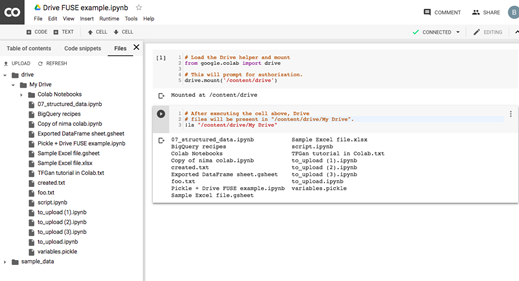
\includegraphics[width=0.8\textwidth]{google_colab_interface}
        \caption{Интерфейс Google Colab}
        \label{fig:google_colab_interface}
    \end{figure}

    Google Colab используется компаниями, такими как Uber и Airbnb, для разработки и обучения моделей машинного обучения, которые помогают оптимизировать маршруты, повышать эффективность работы водителей, предсказывать спрос на жилье и определять цены на аренду.

    Google Colab использует Jupiter—ноутбуки – среда разработки, в которой написанный код выполняется блоками. Такая среда разработки является удобной и имеет ряд преимуществ:
    \begin{enumerate}
        \item Удобство. Jupyter—ноутбук — среда разработки, где сразу можно видеть результат выполнения кода и его отдельных фрагментов. Отличие от традиционной среды разработки в том, что код можно разбить на куски и выполнять их в произвольном порядке;
        \item Наглядность. Все находится в одном месте: код, сопровождающий текст, результаты и визуализация. Поэтому нужная информация всегда под рукой, а оформить ее можно в понятном формате. При этом Jupiter — полноценная среда, в которой можно запускать код и проверять его;
        \item Документоориентированность. Jupyter Notebook позволяет создавать интерактивные документы, которые могут включать код, текст, графики и другие элементы. Благодаря такому отображению с его помощью можно создавать интерактивные документы по работе или для обучения;
        \item Широкие возможности. Jupyter Notebook поддерживает большое количество языков программирования, в том числе специфических, имеет необходимые разработчику библиотеки. Облачная версия предоставляет мощности для отрисовки графиков — их тоже можно визуализировать с помощью разных инструментов. Markdown позволяет делать документы красивее и форматировать их. Есть поддержка расширений: для создания презентаций, экспортирования документов в HTML и прочих функций;
        \item Моментальный вывод результата. Результат выполненной программы в стандартной IDE открывается в отдельном окне или записывается в файл. В любом случае его довольно редко бывает можно просмотреть внутри среды, если это не текст и не число, а, скажем, график или таблица. А в Jupyter Notebook все отображается сразу под кодом, в том же документе;
        \item Командная работа. Возможности для командной работы позволяют делиться документом с другими, запускать собственный сервер для группы разработчиков, совместно редактировать и исправлять ошибки. Все это в одной и той же версии документа, а не в разных его экземплярах (как было бы, например, с передачей друг другу файлов с кодом).
    \end{enumerate}

    Платформа Google Colab использует мощности Google Cloud, включая графические процессоры (Graphic Processing Unit, GPU) и тензорные процессоры (Tensor Processing Unit, TPU). Такое техническое оборудование необходимо для относительно быстрого и эффективного выполнение задач машинного обучения, по сравнению с применением обычного СPU (Central Processing Unit). Относительность, однако, заключается в высоконагруженных задачах обучения математических моделей – чем сложнее алгоритм, тем дольше он будет вычисляться.

    В качестве GPU платформа использует различные видеокарты, включая NVIDIA Tesla K80, T4, P4 и P100. Для CPU Google Colab использует процессоры от компании Intel, такие как Intel Xeon, Intel Core i7 и Intel Core i9. Конкретная видеокарта или процессор, который будет использоваться, зависит от доступности в момент использования.

    Использование устройств компании NVIDIA в Google Colab неспроста. Применение GPU лучше подходит для задач машинного обучения, чем CPU, поскольку GPU имеет большое количество ядер и способен обрабатывать большое количество данных параллельно. Устройства NVIDIA имеют технологию CUDA — программную платформу, которая позволяет использовать возможности GPU для вычислений общего назначения. Эта технология дает разработчикам доступ к вычислительной способности графического процессора, который обладает высокой эффективностью при решении многопотоковых задач. Таким образом, использование GPU и технологии CUDA позволяет значительно ускорить процесс обучения нейронных сетей и повысить эффективность работы модели.
    
    TPU – это специализированный процессор, разработанный компанией Google для ускорения машинного обучения и глубокого обучения. Использование TPU ускоряет вычисления с тензорами. Тензоры — это многомерные массивы, используемые в программировании для хранения и обработки данных. Они являются основным типом данных в библиотеках глубокого обучения, таких как TensorFlow и PyTorch. Тензоры могут иметь любое количество измерений (например, одномерный массив, двумерная матрица или трехмерный объем) и хранить числа любого типа (например, целые числа или числа с плавающей точкой). Они используются для представления данных, таких как изображения, звуковые файлы и текстовые документы. У процессора TPU в разы выше производительность при больших объемах вычислительных задач. Google TPU является аппаратным ускорителем, который работает с TensorFlow и другими фреймворками машинного обучения.
    
    Несмотря на множество преимуществ, Google Colab имеет и некоторые недостатки:
    \begin{enumerate}
        \item Ограниченное время работы: Google Colab автоматически отключается после 12 часов бездействия. Это означает, что вы должны перезапустить среду выполнения каждые 12 часов;
        \item Иностранная платформа: Colab является продуктом компании Google, следовательно ее применение в России может быть ограничено. GIT (Global Information Tracker) – система контроля и управления версиями. С ее помощью возможно сравнивать, анализировать, редактировать, вносить изменения и возвращаться назад к последнему сохранению.
    \end{enumerate}

    С помощью утилит Git вы можете вернуть свой проект до более старой версии, сравнивать, анализировать или вносить свои изменения в репозиторий. Репозиторий — это все файлы, находящиеся под контролем версий, вместе с историей их изменения и другой служебной информацией. Существуют разные способы хранения и использования репозитория: выделяют локальные, централизованные и распределенные системы контроля версий. В локальных системах контроля версий репозиторий хранится и используется на одном устройстве, но работать с такой системой может только один разработчик. В случае централизованной системы репозиторий хранится на одном сервере.
    
    Каждая точка сохранения вашего проекта носит название коммит (commit). У каждого коммита есть хэш (hash, уникальный идентификатор или id) и комментарий. Из таких коммитовов собирается ветка. Ветка – это история изменений. Существует два типа веток: постоянные (master—ветка, чтобы понимать, как выглядит последняя актуальная версия, и development—ветка, где ведется разработка) и временные ветки (feature—ветка, для добавления новых возможностей, release—ветка, для работы над новыми версиями, hotfix—ветка, для быстрого исправления багов).
    
    GitHub — это веб—сервис для хостинга и управления репозиториями Git, который предоставляет возможность хранить, управлять и совместно работать над проектами с помощью системы контроля версий. 
    
    Использование Git (в том числе платформы GitHub) позволяет:
    \begin{enumerate}
        \item Отслеживать изменения, произошедшие с проектом со временем. Благодаря этому есть возможность посмотреть как менялись файлы программы, на всех этапах разработки и при необходимости вернуться назад и что—то отредактировать;
        \item Организовать одновременную работу нескольких разработчиков над одним проектом. Без использования Git возможен конфликт, когда разработчики, скопировав весь код из главной директории и сделав с ним задуманное, попытаются одновременно вернуть весь код обратно. Git является распределенным, то есть не зависит от одного центрального сервера, на котором хранятся файлы. Вместо этого он работает полностью локально, сохраняя данные в репозитории. При этом центральный сервер используется для координации работы множества разработчиков над одним проектом. Он является центральным хранилищем для всех изменений, которые вносятся в проект, и позволяет разработчикам синхронизировать свои локальные копии с общим репозиторием.
    \end{enumerate}

    Docker — это открытая платформа для разработки, доставки и эксплуатации приложений. С помощью docker можно отделить приложение от общей инфраструктуры и обращаться с инфраструктурой как управляемым приложением. 
    
    В своем ядре docker позволяет запускать практически любое приложение, безопасно изолированное в контейнере. Безопасная изоляция позволяет запускать на одном хосте много контейнеров одновременно. 
    
    Docker – это платформа работы с контейнерами. Контейнеры позволяют упаковывать приложения и их зависимости в единую среду, которая может быть легко перенесена между различными средами и операционными системами. Docker упрощает процесс разработки и развертывания приложений, ускоряет доставку и повышает надежность работы приложений, так как контейнеры изолируют приложения друг от друга и от хост—системы. Docker также облегчает масштабирование приложений, так как можно легко создавать и удалять контейнеры в зависимости от нагрузки.
    
    Docker использует архитектуру клиент—сервер. Docker клиент общается с демоном (daemon) Docker, который управляет созданием, запуском и распределением контейнеров. Клиент и сервер могут работать на одной системе, есть возможность подключения клиента к удаленному демону docker. Клиент и сервер общаются через сокет или через RESTful API (см. \hyperlink{fig:docker_structure}{Рисунок 8}).

    \begin{figure}[ht]
        \centering
        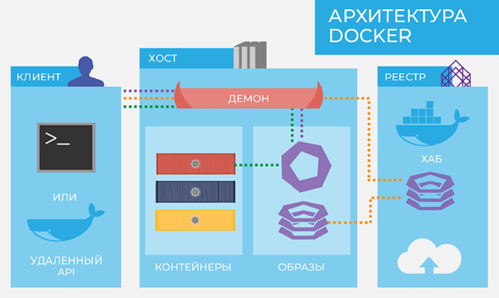
\includegraphics[width=0.8\textwidth]{docker_structure}
        \caption{Структура платформы Docker}
        \label{fig:docker_structure}
    \end{figure}

    С ростом количества Docker—контейнеров их становится труднее поддерживать. Конфигурация каждого контейнера описывается в своем Dockerfile, которые необходимо запускать отдельной командой. Так же возникает проблема сборки или пересборки контейнеров.

    Для облегчения работы с большим количеством контейнеров используется Docker Compose — это инструмент для описания многоконтейнерных приложений. С его помощью можно собрать один файл, в котором наглядно описываются все контейнеры. Еще Docker Compose позволяет собирать, останавливать и запускать файлы одной командой.
    
    Преимущества использования Docker:
    \begin{enumerate}
        \item Изоляция: Docker контейнеры позволяют изолировать приложения и их зависимости от остальной системы, что уменьшает возможность конфликтов и повышает безопасность;
        \item Переносимость: Docker контейнеры могут быть развернуты на любой платформе, поддерживающей Docker, что упрощает процесс развертывания и обновления приложений;
        \item Масштабируемость: Docker позволяет масштабировать приложения горизонтально, что означает, что можно добавлять новые контейнеры для увеличения производительности;
        \item Эффективность использования ресурсов: Docker использует меньше ресурсов, чем традиционные виртуальные машины, что позволяет увеличить эффективность использования серверов;
        \item Упрощение DevOps: Docker позволяет автоматизировать процесс сборки, тестирования и развертывания приложений, что ускоряет процесс разработки и уменьшает количество ошибок.
    \end{enumerate}

    Недостатки использования Docker:
    \begin{enumerate}
        \item Сложность настройки: Настройка Docker может быть сложной задачей, особенно для начинающих пользователей;
        \item Ограниченный доступ к ресурсам хост—системы: Docker контейнеры имеют ограниченный доступ к ресурсам хост—системы, что может привести к проблемам с производительностью;
        \item Необходимость постоянного обновления: Docker постоянно обновляется, и это может требовать дополнительных усилий для обновления и поддержки;
        \item Размер контейнеров: Docker контейнеры могут быть довольно большими, что может привести к проблемам с хранением и передачей контейнеров;
        \item Безопасность: Docker контейнеры могут быть уязвимы для атак, особенно если настроены неправильно.
    \end{enumerate}

    IDE для Python (Integrated Development Environment) — это интегрированная среда разработки, которая облегчает процесс создания программ на языке Python. IDE обычно включает в себя текстовый редактор, инструменты для отладки и тестирования кода, автодополнение кода, подсветку синтаксиса, управление версиями, интеграцию с системами контроля версий и другие полезные функции. Некоторые из самых популярных IDE для Python включают в себя PyCharm, Atom, IDLE и Jupyter Notebook. Каждая из них имеет свои особенности и преимущества, и выбор IDE зависит от предпочтений и потребностей разработчика.

    PyCharm — это интегрированная среда разработки (IDE) для языка программирования Python, разработанная компанией JetBrains. PyCharm предоставляет множество функций и инструментов для упрощения и ускорения процесса создания, отладки и тестирования программ на Python. 
    
    Основные особенности PyCharm включают:
    \begin{enumerate}
        \item Редактор кода: PyCharm обеспечивает удобный и интуитивно понятный текстовый редактор, который поддерживает множество функций, таких как автодополнение кода, подсветка синтаксиса, автоматическое форматирование кода и другие;
        \item Отладчик: PyCharm имеет мощный отладчик, который позволяет легко отслеживать ошибки в коде и исправлять их. Отладчик PyCharm поддерживает множество функций, таких как точки останова, просмотр переменных и стека вызовов, а также возможность изменять значения переменных во время выполнения программы;
        \item Интеграция с системами контроля версий: PyCharm интегрируется с популярными системами контроля версий, такими как Git, Mercurial и Subversion. Это позволяет разработчикам легко управлять своими проектами и отслеживать изменения в коде;
        \item Управление зависимостями: PyCharm позволяет легко управлять зависимостями проекта, используя инструменты, такие как pip и virtualenv. Это позволяет разработчикам управлять версиями библиотек и модулей, которые используются в проекте;
        \item Интеграция с другими инструментами: PyCharm интегрируется с множеством других инструментов и библиотек, таких как Django, Flask, SQLAlchemy, NumPy, SciPy и другие. Это позволяет разработчикам использовать эти инструменты и библиотеки в своих проектах и ускорить процесс разработки;
        \item Jupyter Notebook: PyCharm имеет интеграцию с Jupyter Notebook, что позволяет разработчикам создавать и запускать блокноты Jupyter прямо из среды разработки PyCharm;
        \item Поддержка различных операционных систем: PyCharm доступен для Windows, macOS и Linux, что позволяет разработчикам работать на любой платформе.
    \end{enumerate}

    Интерфейс PyCharm представлен на \hyperref[fig:pycharm_window]{Рисунке 9}.

    \begin{figure}[ht]
        \centering
        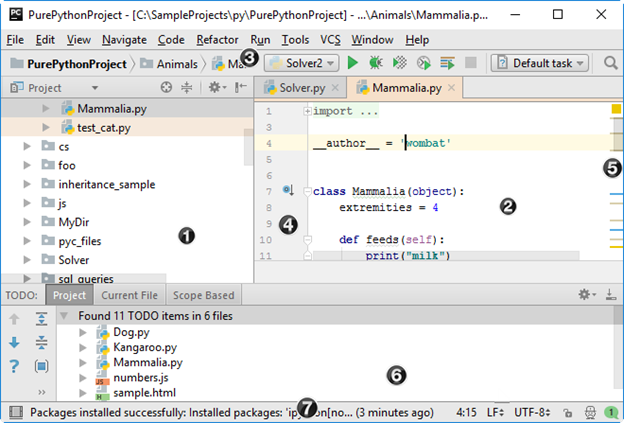
\includegraphics[width=0.8\textwidth]{pycharm_window}
        \caption{Окно разработки в PyCharm}
        \label{fig:pycharm_window}
    \end{figure}

    \begin{enumerate}
        \item Project Tool Window. Панель инструментов проекта. В этом окне отображаются файлы вашего проекта;
        \item PyCharm Editor. Редактор PyCharm. Находится с правой стороны, где вы пишете свой код. В нем есть вкладки для удобной навигации между открытыми файлами;
        \item Navigation Bar. Панель навигации. Находится над редактором, позволяет быстро запускать и отлаживать ваше приложение, а также выполнять процедуры контроля версий VCS;
        \item Left gutter. Левый столбец, вертикальная полоса рядом с редактором, показывает брекпоинты и обеспечивает удобный способ перехода по иерархии кода. Он также отображает номера строк и историюVCS;
        \item Right gutter. Правый столбец, справа от редактора. PyCharm постоянно контролирует качество вашего кода и постоянно показывает результаты проверки в правом столбце: ошибки, предупреждения и т.д. Индикатор в правом верхнем углу показывает общий статус проверки кода для всего файла;
        \item PyCharm Tool Windows. Панель инструментов PyCharm. Это специальные окна, прикрепленные к низу и сторонам рабочей области, которые обеспечивают доступ к типичным задачам, таким как управление проектами, поиск и навигация по исходному коду, интеграция с системами контроля версий и т.д;
        \item Status Bar. Строка состояния. Указывает состояние вашего проекта и показывает различные предупреждения и информационные сообщения.
    \end{enumerate}    

    Как и любой продукт, PyCharm имеет свои недостатки, включая:
    \begin{enumerate}
        \item Высокие требования к системным ресурсам: PyCharm может потреблять много оперативной памяти и процессорного времени, особенно при работе с большими проектами;
        \item Сложность для новичков: PyCharm может быть сложным для новичков, которые только начинают изучать язык программирования Python. Некоторые функции и инструменты могут быть непонятными или непригодными для начинающих разработчиков;
        \item Платная версия: Professional Edition PyCharm является платной, что может быть недоступно для некоторых разработчиков, особенно для студентов или новичков;
        \item Ограниченная поддержка других языков: PyCharm специализируется на языке программирования Python и может быть не так полезен для разработки программ на других языках;
        \item Некоторые функции могут быть неустойчивыми: Некоторые функции и инструменты PyCharm могут быть неустойчивыми или не работать должным образом в некоторых случаях, что может вызвать проблемы при разработке программ.
    \end{enumerate}

    Подытожив, можно сказать, что данная платформа, хоть и имеет некоторые недостатки, но всё же является лучшим выбором для работы на языке Puthon, т.к. структурирована и создана под конкретный язык.

    \section{Состояние и перспективы технологий машинного обучения и анализа данных}
    Машинное обучение (ML) — это одно из самостоятельных центральных направлений искусственного интеллекта (ИИ), сосредоточенное на создании систем, которые обучаются и развиваются на основе получаемых ими данных. Общая цель машинного обучения — разработка программ, которые могут учиться на основе данных и делать прогнозы на основе результатов этого обучения.

    Начальные данные для машинного обучения (входные данные) называются датасетом (Dataset). К данным, необходимым для машинного обучения, относятся объекты, признаки и ответы. Реализация процесса машинного обучения построена на нахождении алгоритма, шаблона или зависимости  преобразования входных данных в выходные данные (ответы) по признакам. 
    
    Состояние и перспективы технологий машинного обучения и анализа данных в области интеллектуальных технических систем являются ключевыми и обещают значительный прогресс в различных сферах применения. В настоящее время мы наблюдаем значительный рост интереса к этим технологиям и их активное применение в различных отраслях, таких как здравоохранение, автомобильная промышленность, финансы, энергетика и другие.
    
    Состояние технологий машинного обучения и анализа данных на сегодняшний день обладает характерными отличительными чертами. Одной из главных особенностей является возможность обучения моделей на больших объемах данных. Возможность использования огромных наборов данных, собранных из различных источников, позволяет создавать более точные и обобщающие модели, способные решать сложные задачи.
    
    Машинное обучение подразумевает процесс анализа данных программой или алгоритмом с определением признаков и закономерностей для решения последующих аналогичных задач. Основная масса задач, решаемых при помощи методов машинного обучения, относится к двум разным видам: обучение с учителем (supervised learning) либо без него (unsupervised learning). Однако «учителем» называется выборка данных, которая отображает явным образом правильность обучения и верные ответы при обучении. Учитель – это вмешательство человека в надстройке путей решения по конечному результату. В обоих видах обучения машине предоставляются исходные данные, которые ей предстоит проанализировать и найти закономерности. Различие лишь в том, что при обучении с учителем есть ряд гипотез, которые необходимо опровергнуть или подтвердить.
    
    Методы глубокого машинного обучения:
    \begin{enumerate}
        \item Контролируемое обучение. Машине задаются входные данные и их предпочтительные выходы, объекты, называемые «учителем», и цель состоит в том, чтобы изучить общее правило, которое отображает входные данные для выходов. Эти алгоритмы применяют все, что они узнали ранее, к любым новым данным;
        \item Неконтролируемое обучение. Метки / теги или объяснения не даются алгоритму обучения в отношении ввода, и он остается сам по себе, чтобы найти в нем структуру. Используется для обнаружения скрытых шаблонов в данных. Эти алгоритмы могут извлекать свои собственные выводы или выводы из данных наборов данных;
        \item Обучение в действии. Программное обеспечение взаимодействует с изменяющейся средой, в которой она должна выполнять определенную задачу (например, вождение транспортного средства), не сообщая, приближается ли она к ее месту назначения или узнает, как играть в игру, играя против кого—то;
        \item Полууправляемое машинное обучение. Субъект «учитель» дает машине данные с некоторыми недостатками, выходы отсутствует.
    \end{enumerate}

    Развитие методов глубокого обучения с подкреплением представляет собой значимый прорыв в области машинного обучения и анализа данных. Эти методы позволяют моделям обучаться, взаимодействуя с окружающей средой и получая обратную связь на основе своих действий. Они находят широкое применение в различных областях, включая робототехнику, игровую индустрию, финансовый сектор и многие другие.

    Одним из ключевых аспектов глубокого обучения с подкреплением является возможность создания автономных систем, способных принимать решения и выполнять действия в реальном времени. Модели, обученные с использованием этого подхода, могут адаптироваться к изменяющейся среде, обучаться на основе своего опыта и принимать оптимальные решения для достижения поставленных целей. Это открывает перспективы для создания автономных роботов, умных систем управления и других технических решений, которые могут успешно функционировать в разнообразных и динамических средах.
    
    Еще одной важной характеристикой методов глубокого обучения с подкреплением является их способность к обучению на основе награды. Модели стремятся максимизировать получаемую награду, что позволяет им находить оптимальные стратегии и принимать решения, которые приводят к наилучшему результату. Это открывает возможности для применения этих методов в задачах оптимизации, управления, планирования и других областях, где необходимо достичь определенной цели с учетом внешних условий и ограничений.
    
    Перспективы развития методов глубокого обучения с подкреплением обещают быть весьма впечатляющими. Ожидается, что будут разработаны более сложные и эффективные алгоритмы, позволяющие моделям учиться на основе более сложных иерархических структур данных.
    
    Развитие более эффективных алгоритмов обучения является важной задачей, поскольку они определяют способность моделей к обобщению и принятию точных решений на основе данных. Усовершенствованные алгоритмы могут обеспечить более высокую точность и скорость обучения моделей, а также повысить их устойчивость к шуму и изменчивости данных.
    
    Другим важным аспектом состояния технологий машинного обучения и анализа данных является применение глубоких нейронных сетей. Эти архитектуры моделей позволяют эффективно работать с изображениями, текстами и звуками, распознавать образы, классифицировать данные и выполнять другие сложные задачи.
    
    Искусственные нейронные сети представляют собой систему (математическую модель) соединённых и взаимодействующих между собой простых процессоров (искусственных нейронов). Данная модель, а также её программное или аппаратное воплощение, построенная по принципу организации и функционирования биологических нейронных сетей — сетей нервных клеток живого организма. Представляют собой сеть элементов — искусственных нейронов — связанных между собой синаптическими соединениями. Сеть обрабатывает входную информацию и в процессе изменения своего состояния во времени формирует совокупность выходных сигналов. Работа сети состоит в преобразовании входных сигналов во времени, в результате чего меняется внутреннее состояние сети и формируются выходные воздействия. Сравнение искусственного нейрона с биологическим носит лишь пояснительный характер для более точного пояснения работы, как по примеру электромеханической аналогии для колебательных систем и других.
    
    В целом, при рассмотрении нейронных сетей стоит обратить внимание на структуру искусственного нейрона. Нейрон имеет следующую структуру, представленную на \hyperref[fig:artificial_neuron_structure]{Рисунке 10}.

    \begin{figure}[ht]
        \centering
        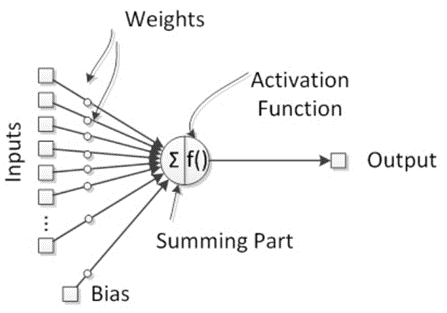
\includegraphics[width=0.8\textwidth]{artificial_neuron_structure}
        \caption{Структура искусственного нейрона}
        \label{fig:artificial_neuron_structure}
    \end{figure}

    Как показано на рисунке 1.14, нейрон имеет входы (inputs), получающие исходный сигнал и данные, т.е. принимают исходный вектор, кодирующий входной сигнал. Входной сигнал проходит в сумматор (summing part) через веса (weights). Веса в искусственном нейроне – это определенный коэффициент, влияющий на величину сигнала, пришедшего в сумматор. Веса отражают «важность» входного сигнала, определяют его влияние на результат работы нейрона. Возможность изменения весов предоставляет возможность изменения работы и действия нейрона, его выходного сигнала (output). Биас (bias) — сдвиг относительно оригинального значения. В нейронных сетях используется как добавочный коэффициент к взвешенной сумме входных сигналов нейрона. Сумматор в нейронных сетях – это блок, суммирующий сигналы, поступающие от нейронов через синапсы. В общем случае сумматор может преобразовывать сигналы и передавать их нейронам или сумматорам тоже через синапсы. Исходя из активационной функции и взвешенной суммы, полученной на сумматоре по входным сигналам с учетом их весов, определяется значение сигнала подаваемого на выход. 
    
    Глубокие нейронные сети и сверточные нейронные сети стали важными инструментами в области машинного обучения и анализа данных. Они представляют собой архитектуры моделей, вдохновленные работой человеческого мозга, и способны обрабатывать сложные иерархические структуры данных.
    
    Иерархическая структура нейронной сети называется архитектурой нейронной сети. Основные архитектуры современных нейросетей представлены на рисунке.
    
    На \hyperref[fig:artificial_neural_networks_architecture]{Рисунке 11} представлены некоторые типы искусственных нейронов, рассмотрим их подробнее:

    \begin{enumerate}
        \item Входные нейроны (input cell) — принимают исходный вектор, кодирующий входной сигнал. Как правило, эти нейроны не выполняют вычислительных операций, а просто передают полученный входной сигнал на входы нейронов следующего слоя;
        \item Возвращающие входные нейроны (backfed input cell) – могут как принимать сигнал, так и использоваться при регистрации выхода;
        \item Зашумленный входной нейрон (noisy input cell) – принимает искаженный входной сигнал;
        \item Бинарный скрытый нейрон (hidden cell) – производит основные операции преобразования входного сигнала, может обладать различными механизмами и фильтрами;
        \item Скрытый нейрон (probabilistic hidden cell) с вероятностной интерпретацией входного сигнала;
        \item Зашумленный (импульсный) скрытый нейрон (spiking hidden cell) – третье поколение искусственных нейронов, которое отличается от бинарных и частотных/скоростных нейронов тем, что в нем нейроны обмениваются короткими импульсами одинаковой амплитуды.
        \item Капсульные скрытые нейроны (capsule cell), содержащие капсулу – элемент, являющихся промежуточной единицей между нейроном и слоем, который представляет собой группы виртуальных нейронов, отслеживающих не только отдельные детали изображения, но и их расположение друг относительно друга
        \item Выходные нейроны (output cell) — представляют выходы сети. В выходных нейронах могут производиться вычислительные операции суммирования и определения значения активационной функции;
        \item Совпадающие нейроны входа—выхода (match input output cell), по аналогии с возвращающими нейронами, однако отличие в том, что на нейроны 2 сначала подается сигнал, и входе работы НС может регистрироваться выход, а на нейронах входа—выхода корректируется работа НС по полученному выходу, подавая входной сигнал;
        \item Рекуррентные нейроны (recurrent cell), или же нейроны обратной связи, позволяют менять состояние нейрона, используя как сигнал от предыдущего слоя, так и свое состояние в предыдущий момент времени;
        \item Нейрон памяти (memory cell), «запоминает» определенное состояние и может передавать его в качестве сигнала. Можно сравнить с ОЗУ ПК;
        \item Закрытый нейрон памяти (gated memory cell), записывает сигнал, полученный на входе, и может им обмениваться в любой момент времени. Можно сравнить с ПЗУ;
        \item Ядро (kernel), или же элемент фильтра свертки, представляет собой механизм конвертации и генерирует матрицы свертки;
        \item Сверточный нейрон или пулинг—нейрон (convolution or pool), в зависимости от архитектуры представляет собой нейрон слоя свертки или объединения, соответственно позволяет либо обобщение данных в процессе свертки с уменьшением размерности, либо для извлечения доминирующих признаков и работой с инвариантностью;
    \end{enumerate}

    \begin{figure}[ht]
        \centering
        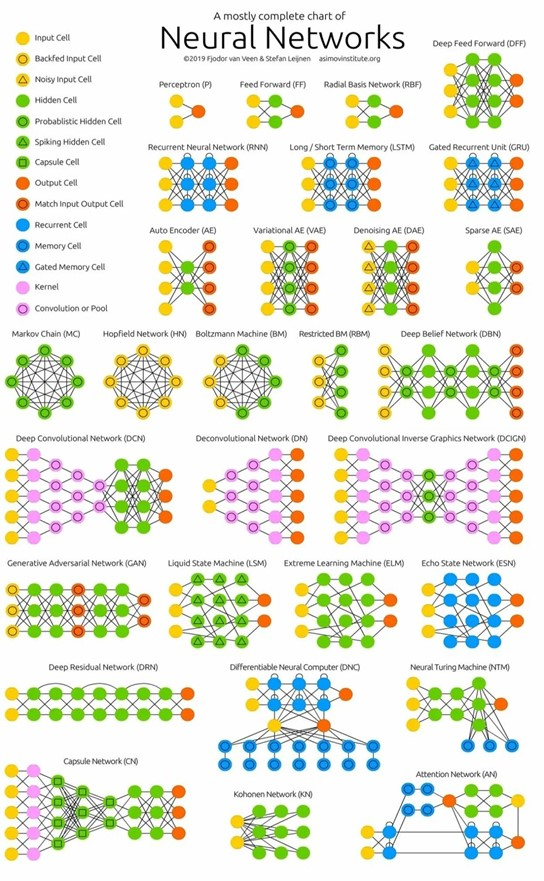
\includegraphics[width=0.5\textwidth]{artificial_neural_networks_architecture}
        \caption{Архитектуры искусственных нейронных сетей}
        \label{fig:artificial_neural_networks_architecture}
    \end{figure}

    Нейронные сети принято классифицировать следующим образом: сети прямого распространения и рекуррентные нейросети (с обратной связью), полносвязные и неполносвязные сети (по соединению нейронов в слое между собой и другими слоями), глубокие и неглубокие сети (если больше 2х скрытых слоев – глубокие).
    
    Нейронные сети прямого распространения являются сетями представляющими собой ориентированный ациклический граф. Ациклический означает, что у него нет замкнутых петлевых отношений.
    
    Элементарный персептрон, используется для вычисления простых (бинарных) логических значений. Данная архитектура может заменить логические операторы AND и OR. Имеет входной слой и выходной, сеть выдает сигнал на выходе, если сигнал какого либо из нейронов входного слоя с учетом веса связи слоев превысил какое либо пороговое значение.

    Персептрон с одним скрытым слоем (или же сеть прямого распространения), архитипичная модель нейронной сети, представляет собой структуру из трех типов элементов: рецепторов (сенсоров), ассоциативных и реагирующих. Для данных элементов более применительно использование следующей терминологии: входные, скрытые и выходные элементы. Несколько параллельных элементов одного типа называются слоями. Элементы скрытого слоя для перцептрона называются ассоциативными, т.к. каждому элементу соответствует целый набор элементов входного слоя (рецепторов). Элементы ассоциативного слоя могут иметь всего 2 состояния – состояние покоя и возбуждения. Элемент активизируется, если на его входе количество сигналов от предыдущего слоя превысило некоторую величину. В случае персептрона, если элемент ассоциативного слоя активизирован, то он передает сигнал на выходной слой, или же сумматор. Сумматор подсчитывает сумму значений входных сигналов, помноженных на веса (линейную форму). Элементарный перцептрон в таком случае выдаёт «1», если линейная форма превышает порог, иначе на выходе будет «−1». Математически функцию, реализуемую на сумматоре, можно записать так \hyperref[eq:eq1]{(см. Формулу 1)}:

    \begin{equation}
        f(x)=\operatorname{sign}\left(\sum_{i=1}^n w_i x_i-\theta\right)
        \label{eq:eq1}
    \end{equation}

    Ассоциативный элемент – обычный нейрон модели МакКаллока—Питса с бинарно—пороговой функцией активации. Реагирующий элемент – обычный нейрон с биполярно—пороговой функцией активации. Персептрон является простейшей сетью прямого распространения — линейным классификатором. Модель перцептрона в основном подходит для решения задач классификации, однако может применяться для прогнозирования и распознавания образов. 

    Радиальная базисная сеть, имеет схожую структуру с персептроном, однако отличие заключается в функциях активации. Функция активации в персептроне обеспечивает глобальную аппроксимацию нелинейного отображения, в радиальной базисной сети – при помощи экспоненциально уменьшающихся локализованных нелинейностей (т.е. функций Гаусса) создается локальная аппроксимация нелинейного отображения. Радиальная базисная сеть обычно используются для задач аппроксимации. Эта сеть обладает высокой скоростью обучения. 
    
    Глубокая сеть прямого распространения, имеет несколько скрытых слоев, что повышает вычислительную мощность. 
    
    Автоинкодер – его цель восстановить входной сигнал на выходе. Поэтому автоэнкодеры используют для нахождения общих закономерностей в данных, а также для восстановления исходных данных из сжатых. Скрытый слой данных НС имеет размерность меньшую, чем у входного и выходного слоев. Если сигнал, сгенерированный на выходе равен сигналу, принятому на входе, значит среднего слоя, с меньшей размерностью, достаточно для описания входа. В качестве полезного используют именно средний слой. Автоэнкодер можно рассматривать как обобщение методов линейного понижения размерности. Данная архитектура успешно проявляет себя в задачах архивации и шифрования и наоборот. Пример: если разбить автоинкодер попалам, то можно использовать входную часть для кодировки информации, а выходную для расшифровки.
    
    Разреженный автоинкодер. Данная нейросеть намеренно увеличивает степень разреженности скрытых нейронов на этапе обучения, притом, что скрытых нейронов больше, чем выходов, чтобы сеть могла обучиться распознаванию полезных структур в данных. Обычно разреженность реализуется пороговым отсечением. Сеть имеет большее количество нейронов на скрытом слое, чем на входном и выходном, однако нейроны скрытого слоя имеют разряженную активацию. Разреженная активация – это превышение количества неактивных нейронов относительно активных. Для предотвращения копирования сигналов между слоями используется метод ошибки обратного распространения.
    
    Вариационный автоэнкодер использует вероятностный подход для описания наблюдений. Он показывает распределение вероятностей для каждого атрибута в наборе функций. Данная нейросеть зачастую обучается алгоритмами градиентного спуска, что позволяет выводить предположения о распределении латентных переменных и использовать сеть для прогнозирования. Иными словами, подобные нейросети генерируют новые данные на выходе из вариации данных на входе. Принадлежит к семействам вероятностных графических моделей и вариационных байесовских методов.
    
    Шумоподавляющий автоинкодер. Данная нейросеть принимает частично искаженные обучающие входные данные и пытается восстановить исходный сигнал. Искажение (или же шум) специально добавляется к входу, чтобы обучить сеть нелинейному погружению. Подобная архитектура появилась при решении проблемы идентификации данных. В конечном счете, можно сказать, что НС используя функцию потерь, снимает шум с исходных данных. Самыми распространенными функциями потерь для сети являются среднеквадратическая ошибка (MSE) или двоичная кросс‑энтропия.
    
    Сеть Хопфилда представляет базовую архитектуру полносвязной сети, каждый нейрон которой может играть роль входа (сделано для того, чтобы нейросеть не зависела от порядка входных данных). Сеть является обучаемой системой ассоциативной памяти, адресуемой по содержимому, с бинарными пороговыми блоками. Входные данные продвигаются по сети, причем гарантируется сходимость к локальному минимуму. Иногда решение сходится к ложному паттерну (неправильноному локальному минимуму), а не к хранимому (ожидаемому локальному минимуму). Сети свойственно сложное обучение и низкая вычислительная мощность. Взаимодействие нейронов описывается следующим образом \hyperref[eq:eq2]{(см. Формулу 2)}:

    \begin{equation}
        E=\frac{1}{2} \sum_{i, j=1}^N w_{i j} x_i x_j
        \label{eq:eq2}
    \end{equation}

    Отличие обучения сети Хопфилда заключается в том, что вместо последовательного приближения к нужному состоянию с вычислением ошибок, все коэффициенты матрицы рассчитываются по одной формуле, за один цикл, после чего сеть сразу готова к работе. Применяется, например, для возращения исходного изображения по искаженному. 

    Цепь Маркова используется для решения задач динамики случайных величин, где каждая итерация – это изменение состояния данных. Сеть Маркова – это графовая модель, в которой множество случайных величин обладает Марковским свойством, описанным неориентированным графом. Марковское свойство заключается в том, что в любой момент времени условное распределение будущих состояний процесса с заданными текущим и прошлыми состояниями зависит только от текущего состояния, но не от прошлых состояний (свойство отсутствия памяти). Случайный процесс с марковским свойством называется марковским процессом. Марковская сеть отличается от другой графовой модели, Байесовской сети, представлением зависимостей между случайными величинами. Она может выразить некоторые зависимости, которые не может выразить Байесовская сеть (например, циклические зависимости); с другой стороны, она не может выразить некоторые другие.
    
    Машина Больцмана, которую иногда называют стохастической сетью Хопфилда со скрытыми блоками, — это стохастический порождающий аналог сети Хопфилда. Это была одна из первых нейронных сетей, способных обучаться представлениям и (при наличии достаточного времени) решать трудные комбинаторные задачи. В отличие от марковских цепей (не имеющих входных блоков) или сетей Хопфилда (в которых все блоки входные), данная нейросеть является гибридом, в котором имеются как входные, так и скрытые блоки. Работа Машины Больцмана напоминает динамику простых физических процессов. Своим названием она обязана распределению Больцмана в статистической механике, которое используется в их функции выборки.
    
    Ограниченная машина Больцмана. Такую сеть называют двунаправленная, т.к. из входного слоя идет подача на скрытый, и со скрытого на входной. В этой архитектуре связи существуют только между скрытыми и видимыми нейронами, но при этом отсутствуют между нейронами одного класса. Ограниченные машины Больцмана используются в сетях глубинного обучения. 
    
    Глубокая сеть доверия – порождающая графическая модель, состоящая из нескольких слоев скрытых переменных со связями между слоями, но не между блоками одного слоя. Обучение можно производить послойно, начиная со слоя автоэнкодера или ограниченной машины Больцмана (т.к. сеть представляет собой последовательно подключенные автоэнкодеры или органиченные машины Больцмана). Таким образом, каждый слой должен только обучиться кодировать предшествующую сеть — по сути дела, это жадный алгоритм обучения для нахождения локально оптимальных решений. Поэтому сеть можно рассматривать как композицию простых сетей, обучаемых без учителя, например ограниченная машина Больцмана и аавтоэнкодер, в которой скрытый слой каждой подсети играет роль видимого слоя для следующей подсети. Глубокая сеть доверия является одной из первых архитектур глубоких нейросетей, однако с их появлением возникла проблема потери сигнала между слоями (проблема затухающего градиента – производной сигнала).
    
    Глубокая остаточная сеть. Данная архитектура появилась при разработке решения проблемы затухания сигнала. Глубокая остаточная сеть – это глубокая сеть прямого распространения, в которой связи существуют не только между соседними слоями, но и между слоями, отстоящими друг от друга на 2—5 слоев. Поэтому входной сигнал передается сразу на отдаленный слой. Глубина сети может достигать 150 слоев.
    
    Рекуррентные нейросети, первая попытка дать нейросетям память, однако не имеющие механизма сброса состояния. Имеет рекуррентные нейроны. Рекуррентный нейрон в скрытом слое получает помимо информации с предыдущего слоя информацию о своем состоянии в предыдущий момент времени. Данные сети характеризуются тем, что связи между блоками образуют ориентированный граф, вытянутый в одном направлении. Это позволяет моделировать поведение временной последовательности. В отличие от сетей прямого распространения, данная сеть может использовать свое внутреннее состояние (память) для обработки последовательности событий. В канонической архитектуре данных нейросетей каждый нейрон соединен петлей обратной связи с самим собой. Это позволяет оценивать и организовывать временные задержки и контуры обратной связи. Проблема этой нейронной сети — низкая скорость обучения. А также она не хранит давнюю информацию, т.е. не работает с учетом долгосрочной перспективы. Так, управляемые состояния, называемые вентильными или вентильной памятью, служат основой для двух важнейших архитектур: сетей с долгой краткосрочной памятью (long—short term memory — LSTM) и вентильных рекуррентных блоков (gated recurrent units — GRU). 
    
    LSTM сети (сети с долгой краткосрочной памятью), используют LSTM нейроны, внутри каждого нейрона имеются механизмы, а именно фильтры \hyperref[fig:neuron_structure_using_internal_filters]{(см. Рисунок 12)}: 1 – фильтр обнуления, 2 – фильтр обновления, 3 – вывода.

    \begin{figure}[ht]
        \centering
        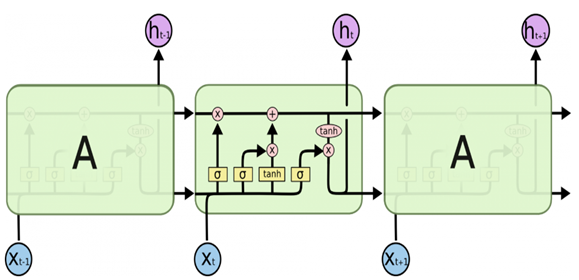
\includegraphics[width=0.5\textwidth]{neuron_structure_using_internal_filters_1}
        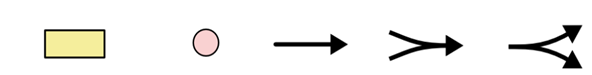
\includegraphics[width=0.5\textwidth]{neuron_structure_using_internal_filters_2}
        \caption{Структура нейрона с применением внутренних фильтров}
        \label{fig:neuron_structure_using_internal_filters}
    \end{figure}    

    На схеме выше каждая линия переносит целый вектор от выхода одного узла ко входу другого. Розовыми кружочками обозначены поточечные операции, такие, как сложение векторов, а желтые прямоугольники – это обученные слои нейронной сети. Сливающиеся линии означают объединение, а разветвляющиеся стрелки говорят о том, что данные копируются и копии уходят в разные компоненты сети.
    
    Управляемая рекуррентная сеть, модификация LSTM, нейроны в данной нейросети имеют всего два фильтра: сброса и обновления. Ее проще обучать, менее громоздка, меньшая вычислительная нагрузка. Управляемые рекуррентные нейроны, в которых фильтры сброса и обновления объединяют в один фильтр \hyperref[fig:controlled_recurrent_neuron_structure]{(см. Рисунок 13)}. Кроме того, состояние ячейки объединяется со скрытым состоянием, есть и другие небольшие изменения. Построенная в результате модель проще, чем стандартная LSTM.

    \begin{figure}[ht]
        \centering
        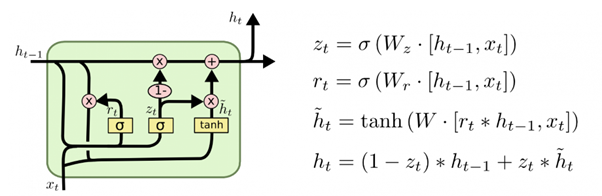
\includegraphics[width=0.8\textwidth]{controlled_recurrent_neuron_structure}
        \caption{Структура управляемого рекуррентного нейрона}
        \label{fig:controlled_recurrent_neuron_structure}
    \end{figure}

    Глубокая сверточная сеть имеет несколько скрытых слоев, которые после входа сжимают информацию, далее полносвязный слой, который обрабатывает уже сжатую информацию и выдает результат. Сверточная сеть, в отличии от предыдущих сетей, состоит из сверточных фильтров и матриц объединения, сверточный фильтр сворачивает квадратный блок изображения в точку, а матрица объединения выбирает максимальное значение. Иерархия архитектуры (послойная) представлена на \hyperref[fig:deep_convolutional_neural_network_layered_structure]{(Рисунке 14)}.
    
    \begin{figure}[ht]
        \centering
        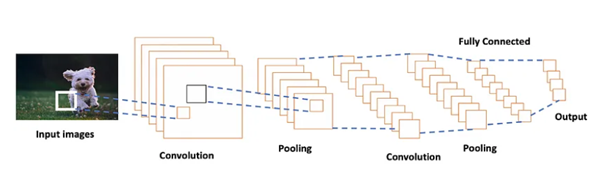
\includegraphics[width=0.8\textwidth]{deep_convolutional_neural_network_layered_structure}
        \caption{Слоистая структура глубокой сверточной нейросети}
        \label{fig:deep_convolutional_neural_network_layered_structure}
    \end{figure}

    Ключевым моментом в понимании сверточных нейронных сетей является понятие так называемых «разделяемых» весов, т.е. часть нейронов некоторого рассматриваемого слоя нейронной сети может использовать одни и те же весовые коэффициенты. Нейроны, использующие одни и те же веса, объединяются в карты признаков (feature maps), а каждый нейрон карты признаков связан с частью нейронов предыдущего слоя. При вычислении сети получается, что каждый нейрон выполняет свертку (операцию конволюции) некоторой области предыдущего слоя (определяемой множеством нейронов, связанных с данным нейроном). Слои нейронной сети, построенные описанным образом, называются сверточными слоями. Помимо, сверточных слоев в сверточной нейронной сети могут быть слои субдискретизации (выполняющие функции уменьшения размерности пространства карт признаков) и полносвязные слои (выходной слой, как правило, всегда полносвязный). Все три вида слоев могут чередоваться в произвольном порядке, что позволяет составлять карты признаков из карт признаков, а это на практике означает способность распознавания сложных иерархий признаков.

    Свертка происходит следующим образом:
    \begin{enumerate}
        \item поданные на вход данные представляются в виде массива чисел или массива матриц чисел;
        \item далее фильтр свертки, который представляет собой матрицу проходит по данным с определенным шагом, перемножая и суммируя исходную матрицу с матрицей фильтра;
        \item следом все каналы свертки (грубо говоря места, где прошелся фильтр) объединяются в общий тензор, который и представляет собой свернутые данные и выражается новой матрицей.
    \end{enumerate}
    
    После свёрточного слоя идёт слой пулинга. Из признаков, которые выделил свёрточный слой, выбирает самые важные, а несущественные удаляет. К результату, который получился во время пулинга, можно снова применить свёрточный слой и сделать несколько циклов. Это нужно, чтобы выстроить иерархию признаков. Первые слои представляют экстрактор, который извлекает сначала низкоуровневые признаки, вплоть до высокоуровневых (детальных) признаков.
    
    Последний свёрточный слой связан с полносвязным слоем, который используется для применения подходящей функции—активатора для прогнозирования выхода: для бинарных выходов используется сигмоидная, а для небинарных — многопеременная функция.
    
    Количество нейронов на слоях выбирается исходя из количества признаков. Для создания исходных матриц также используются признаки, например если необходимо свернуть и проанализировать изображение, то в качестве начального признака может служить интенсивность цвета (яркость) пикселя по RGB шкале.
    
    Развертывающая сеть, по сути, производит операции в обратном порядке. Основным различием между предыдущей сетью и данной является то, что в сверточной входной сигнал подвергается нескольким слоям свертки и субдискретизации. Данная сеть же наоборот стремится сгенерировать входной сигнал в виде суммы сверток карт признаков с учетом применяемых фильтров. Для решения данной задачи, используется широкий спектр инструментов теории распознавания образов, например алгоритмы устранения размытости (deblurring).
    
    Глубокая сверточная сеть обратной графики — разновидность вариационного автокодировщика (VAE), в которой для кодирования и декодирования используются DCNN (сверточные фильтры). Как и в случае автоэнкодеров, выходной слой должен соответствовать входному. 
    
    Капсульная сеть, модификация сверточных сетей, вместо матриц объединения применяются капсулы. Капсулы инкапсулируют информацию о состоянии функции, которую обнаруживают в векторной форме. Капсулы кодируют вероятность обнаружения объекта как длину выходного вектора. Состояние обнаруженной функции кодируется как направление, в котором указывает вектор («параметры создания экземпляра»). Поэтому, когда обнаруженная функция перемещается по изображению или состояние изображения изменяется, вероятность остается неизменной (длина вектора не изменяется), но ориентация меняется. Капсульные нейроны используют следующую нелинейную функцию активации \hyperref[eq:eq3]{(см. Формулу 3)}:

    \begin{equation}
        \mathbf{v}_j=\frac{\left\|\mathbf{s}_j\right\|^2}{1+\left\|\mathbf{s}_j\right\|^2} \frac{\mathbf{s}_j}{\left\|\mathbf{s}_j\right\|}
        \label{eq:eq3}
    \end{equation}

    Правая часть уравнения (синий прямоугольник) масштабирует входной вектор так, что вектор будет иметь длину блока, а левая сторона (красный прямоугольник) выполняет дополнительное масштабирование.

    Генеративно—состязательная нейросеть (порождающая состязательная сеть). Придуманная сравнительно недавно, архитектура порождающей состязательной сети (Generative Adversarial Network), позволяет одновременно обучать две сети. Эти сети часто представляют собой комбинацию DCNN с сетями прямого распространения. В процессе обучения одна сеть порождает данные, а вторая пытается их оценивать. Вообще, порождающая сеть обучается отображать латентное пространство в некоторое представляющее интерес распределение данных, тогда как дисккриминальная сеть различает примеры, выбранные из истинного распределения, и кандидаты, созданные генератором. Цель обучения порождающей сети — увеличить частоту ошибок дискриминантной сети (т. е. «обмануть» дискриминантную сеть, синтезируя примеры, которые выглядят в точности как настоящие – успех одной сети порождает провал другой).
    
    Нейронная Тьюрингова машина. Данная сеть реализует контроллер на основе нейросети, взаимодействующий с внешней памятью посредством механизмов внимания. Взаимодействия с памятью дифференцируемы, поэтому их можно оптимизировать методом градиентного спуска. Данная сеть с LSTM—контроллером может выводить простые алгоритмы, например копирование, сортировку и ассоциативный поиск по предъявленным примерам входа и выхода. 
    
    Дифференциальный нейрокомпьютер, представляет собой архитектуру нейронной сети с дополненной памятью, которая обычно является повторяющейся в своей реализации. Сеть имеет рекуррентные полносвязные нейроны, которые могут через входной и выходной нейроны обращаться к долгосрочной памяти.
    
    Сеть внимания, представляет собой архитектуру—трансформер, имеющую ячейки памяти, фильтрующий блок, блок переключения внимания.
    
    Машина экстремального обучения, обладает такой же базовой архитектурой, как LSM, машина экстремального обучения является сетью прямого распространения для классификации, регрессии, кластеризации, разреженной аппроксимации, сжатия и обучения признакам. Она состоит из одного или нескольких скрытых слоев, причем параметры скрытых блоков (не только веса их связей с входными блоками) не нужно настраивать. Этим скрытым блокам можно назначить случайные веса, которые никогда не обновляются, или веса можно унаследовать от предков без изменения. В большинстве случаев выходные веса скрытых блоков обучаются за один шаг, что по существу сводится к линейной модели.
    
    Сеть с эхо—состояниями – это рекуррентная нейронная сеть со скрытым слоем с разреженными связями (обычно количество связей составляет 1\% от числа блоков). Скрытые нейроны обладают памятью, связи и их веса фиксированы и инициализируются случайным образом. Таким образом, как и в случае LSM и ELM, они не образуют четко упорядоченной слоистой структуры. Веса выходных нейронов можно обучить, так чтобы сеть генерировала конкретные временные паттерны. Возможна корректировка связей и весов только между выходным слоем и связанными с ним нейронами.
    
    Машина неустойчивых состояний, похожа на эхо—сеть, однако в ней используются нейроны накопительного типа, в процессе подачи сигнала на вход которых повышается значение в нем, при заполнении передает результат следующему слою. LSM (Liquid State Machine) – частный случай импульсной нейронной сети. LSM состоит из большого количества блоков, каждый из которых получает меняющийся со временем входной сигнал от внешних источников (входов), а также от других блоков. Блоки связаны между собой случайным образом. Благодаря рекуррентной природе связей зависящий от времени входной сигнал преобразуется в пространственно—временной паттерн активации блоков сети. Паттерны активации считываются линейными дискриминантными блоками. В основе этой архитектуры лежит импульсная деятельность нейронов в мозге. Сеть помогает понять, как импульсные нейроны могут участвовать в обработке и дифференциации информации.
    
    Сети Кохонена, называются также самоорганизующимися картами признаков. Они вполне конкурентоспособны в задачах классификации данных без учителя. Входные данные подаются на вход KN, после чего сеть оценивает, какие нейроны похожи на вход. Самоорганизующиеся карты отличаются от других нейросетей тем, что обучение в них соревновательное, а не основанное на исправление ошибок (например, с помощью градиентного спуска и обратного распространения), и тем, как используется функция соседства для сохранения топологических свойств пространства входов. Поэтому KN полезны для визуализации многомерных данных в пространстве низкой размерности.
    
    Применение глубоких нейронных сетей и сверточных нейронных сетей имеет широкий спектр применений. В области компьютерного зрения, эти модели демонстрируют выдающиеся результаты в распознавании и классификации изображений. Они позволяют автоматически выделять важные признаки изображений и строить сложные модели, способные различать объекты, распознавать лица, определять наличие определенных объектов и многое другое.
    
    Текстовые данные также успешно обрабатываются с использованием глубоких нейронных сетей. Эти модели способны анализировать и интерпретировать естественный язык, выполнять машинный перевод, классифицировать тексты, анализировать настроения и многое другое. Благодаря своей способности обрабатывать контекст и сложные зависимости между словами, глубокие нейронные сети открывают новые возможности для автоматического анализа текстовых данных.
    
    Также следует отметить, что применение глубоких нейронных сетей и сверточных нейронных сетей не ограничивается только изображениями и текстами. Они также успешно используются в области обработки звука и речи, обнаружения и распознавания образов, анализа временных рядов и других задач, требующих обработки сложных данных.
    
    Перспективы развития глубоких нейронных сетей и сверточных нейронных сетей в области интеллектуальных технических систем обещают быть еще более впечатляющими. Ожидается, что будут разработаны новые архитектуры моделей, улучшены методы обучения, увеличена эффективность вычислений и расширены области применения. Перспективы включают использование этих моделей для создания автономных систем, роботов, развитие систем умного дома и многое другое.
    
    В целом, состояние и перспективы технологий машинного обучения и анализа данных в области интеллектуальных технических систем демонстрируют их значительный потенциал и влияние на различные сферы жизни и промышленности. Эти технологии продолжат развиваться и привносить новые возможности для автоматизации, оптимизации и принятия решений в различных сферах, что делает их важным фактором в современном информационном обществе.
    
    Еще одной перспективой является развитие гибридных моделей, объединяющих различные методы машинного обучения и анализа данных. Комбинирование разных подходов позволит создавать более мощные и универсальные системы, способные решать сложные и многогранные задачи.
    
    Именно, гибридные модели машинного обучения и анализа данных представляют собой перспективное направление развития. Комбинируя различные методы, такие как глубокое обучение, методы обучения с подкреплением, байесовские модели и другие, можно создать системы с расширенными возможностями и более высокой адаптивностью.
    
    Кроме того, перспективы включают разработку гибридных моделей, комбинирующих различные методы машинного обучения, например, объединение глубокого обучения с подкреплением и методов обучения с учителем. Это позволит создавать модели, обладающие высокой гибкостью и адаптивностью, способные эффективно решать сложные задачи, требующие как обобщенных знаний, так и способности к самообучению.
    
    Гибридные модели позволяют совмещать преимущества разных подходов и компенсировать их ограничения. Например, можно использовать глубокое обучение для извлечения высокоуровневых признаков из данных, а затем применить методы обучения с подкреплением для обучения агента принимать оптимальные решения на основе полученных признаков. Такое сочетание позволяет создавать интеллектуальные системы, способные справляться с большим разнообразием задач и сценариев.
    
    Кроме того, гибридные модели позволяют учесть контекст и специфические особенности задачи. Например, в задачах обработки естественного языка можно комбинировать методы глубокого обучения с методами классического машинного обучения, чтобы достичь более точных и интерпретируемых результатов.
    
    Дальнейшее развитие гибридных моделей будет направлено на поиск оптимальных способов комбинирования различных методов и алгоритмов, а также на разработку эффективных методов обучения и оптимизации для таких моделей. Это позволит создавать более мощные и универсальные интеллектуальные технические системы.
    
    Таким образом, развитие гибридных моделей машинного обучения и анализа данных представляет значительный потенциал для улучшения производительности и результативности интеллектуальных технических систем, расширения их области применения и достижения новых высот в решении сложных задач.
    
    Также перспективой является интеграция машинного обучения и анализа данных с другими передовыми технологиями, такими как расширенная реальность, квантовые вычисления и другие. Сочетание этих технологий может привести к созданию новых, более сложных и универсальных систем, способных оперативно обрабатывать и анализировать большие объемы данных в реальном времени.
    
    Перспективы технологий машинного обучения и анализа данных в области интеллектуальных технических систем также весьма обнадеживающие. Будущее видится в разработке более сложных моделей, способных адаптироваться к изменяющейся среде и учиться на ходу, а также в улучшении методов интерпретации и объяснения принятых решений. Другие перспективы включают применение гибридных моделей, комбинирующих различные методы машинного обучения, и интеграцию с другими передовыми технологиями, такими как робототехника, автономные системы и интернет вещей.
    
    Интеграция машинного обучения и анализа данных с квантовыми вычислениями открывает перспективы для обработки и анализа данных большой размерности, снижения времени обучения моделей и повышения эффективности работы алгоритмов. Квантовые вычисления могут предоставить ускоренные вычислительные возможности для обработки сложных алгоритмов машинного обучения, что поможет в решении задач, требующих больших вычислительных мощностей.
    
    Интеграция с Интернетом вещей (IoT) позволит собирать данные из различных устройств и сенсоров, что создаст огромный объем информации для анализа и принятия решений. Интернет вещей (Internet of Things, IoT) — это множество физических объектов, подключенных к интернету и обменивающихся данными. Концепция IoT может существенно улучшить многие сферы нашей жизни и помочь нам в создании более удобного, умного и безопасного мира. Примеры Интернета вещей варьируются от носимых вещей, таких как умные часы, до умного дома, который умеет, например, контролировать и автоматически менять степень освещения и отопления. Также ярким примером служит так называемая концепция умного предприятия (Smart Factory), которое контролирует промышленное оборудование и ищет проблемные места, а затем перестраивается так, чтобы не допустить поломок. Применение машинного обучения и анализа данных в IoT—системах позволит оптимизировать процессы, улучшить предсказательные возможности и автоматизировать принятие решений в реальном времени.
    
    Таким образом, интеграция машинного обучения и анализа данных с другими передовыми технологиями открывает широкие перспективы для создания более интеллектуальных и эффективных технических систем. Это позволяет преодолеть ограничения каждой отдельной технологии и создать инновационные решения, способные справляться с сложными задачами и достигать новых высот в автоматизации, управлении ресурсами и принятии обоснованных решений.
    
    Перспективы развития технологий машинного обучения и анализа данных в области интеллектуальных технических систем очень обнадеживающие. Одной из главных перспектив является улучшение точности моделей и расширение их области применения. Развитие новых алгоритмов, методов оптимизации и обучения, а также использование больших вычислительных ресурсов и распределенных вычислений позволит создавать более сложные и интеллектуальные системы.
    
    Кроме того, развитие технологий машинного обучения и анализа данных будет способствовать созданию систем с высокой степенью автономности и способности к адаптации. Это означает, что системы будут способны самостоятельно обучаться и улучшать свою производительность на основе получаемого опыта и новых данных.
    
    Важной перспективой для технологий машинного обучения и анализа данных в области интеллектуальных технических систем является развитие методов объяснения и интерпретации моделей. Возможность понимать и объяснять принятые модели и принимаемые ими решения играет важную роль в доверии и принятии этих систем обществом. Развитие методов интерпретации и объяснения позволит создавать более прозрачные и понятные системы, что может быть особенно важным в критических областях, таких как здравоохранение и автономные транспортные средства.
    
    Понимание принципов и логики, на основе которых модели делают свои предсказания и принимают решения, имеет критическое значение в контексте принятия важных решений в реальном мире. Развитие методов объяснимого и интерпретируемого машинного обучения позволит доверять и применять модели в областях, где требуется прозрачность и понятность принимаемых решений.
    
    Развитие методов объяснения и интерпретации моделей включает в себя разработку алгоритмов и техник, которые позволяют понять, какие признаки и факторы оказывают наибольшее влияние на принимаемые решения модели. Примерами таких методов являются методы визуализации важности признаков, анализа чувствительности модели, методы атрибуции и другие.
    
    Развитие методов интерпретации и объяснения моделей позволит создавать более прозрачные и доверительные интеллектуальные технические системы. Они будут способствовать лучшему пониманию принимаемых решений, обеспечивая возможность проверки их корректности и этичности. Это особенно важно в областях, где принимаемые решения могут иметь серьезные последствия, например, в медицине, где объяснение решений поможет врачам и пациентам понять причины диагнозов и рекомендаций.
    
    Таким образом, развитие методов объяснения и интерпретации моделей машинного обучения является перспективным направлением, способным повысить прозрачность, доверие и эффективность Интеллектуальных технических систем, что в конечном счете приведет к их более широкому и успешному применению в различных областях.
    
    Кроме того, развитие технологий машинного обучения и анализа данных в области интеллектуальных технических систем будет сопровождаться развитием соответствующей инфраструктуры и инструментов. Например, разработка более эффективных алгоритмов обучения, платформ для разработки и развертывания моделей, инструментов визуализации данных и систем управления будет играть важную роль в улучшении производительности и доступности этих технологий.
    
    Технологии анализа данных также продвигаются вперед, предоставляя более мощные инструменты для извлечения ценной информации и знаний из больших объемов данных. Методы обработки и анализа данных, такие как статистический анализ, машинное обучение, графовые алгоритмы и анализ временных рядов, позволяют обнаруживать паттерны, тренды и аномалии в данных, что способствует принятию обоснованных решений и оптимизации бизнес—процессов.
    
    Инфраструктура и инструменты поддерживают технологии и делают их наиболее эффективными при разработке и эксплуатации в различных сферах. Несколько ключевых направлений развития инфраструктуры и инструментов связаны с улучшением алгоритмов обучения, созданием платформ для разработки и развертывания моделей, разработкой инструментов визуализации данных и систем управления.
    
    Платформы для разработки и развертывания моделей играют важную роль в применении технологий машинного обучения и анализа данных. Они предоставляют инструменты разработчикам и исследователям для создания, настройки и оптимизации моделей. Развитие таких платформ, включая интеграцию с другими инструментами разработки и управления данными, помогает упростить процесс разработки и ускорить внедрение моделей в реальные интеллектуальные технические системы.
    
    Инструменты визуализации данных имеют важное значение для понимания и интерпретации результатов анализа данных. Развитие более мощных и гибких инструментов визуализации позволяет визуализировать сложные и многомерные данные, а также обнаруживать скрытые закономерности и паттерны. Это способствует более глубокому пониманию данных и помогает принимать информированные решения на основе анализа.
    
    Системы управления, включая системы мониторинга и контроля, также важны для успешного применения технологий машинного обучения и анализа данных в интеллектуальных технических системах. Они обеспечивают сбор и обработку данных в реальном времени, управление моделями и их интеграцию с другими системами. Развитие таких систем управления позволяет создавать интеллектуальные технические системы, способные адаптироваться к изменяющимся условиям и принимать решения на основе актуальных данных.
    
    Таким образом, развитие инфраструктуры и инструментов для машинного обучения и анализа данных является неотъемлемой частью прогресса в области интеллектуальных технических систем. Усовершенствование алгоритмов, создание платформ, разработка инструментов визуализации и систем управления будут способствовать более эффективному использованию этих технологий, повышению производительности и расширению.
    
    Состояние технологий машинного обучения и анализа данных также отражает активное исследование в области искусственного интеллекта. Множество исследовательских работ направлено на создание новых алгоритмов, моделей и методов, которые способны улучшить качество предсказаний, повысить интерпретируемость моделей и справиться с ограничениями текущих подходов.
    
    В целом, состояние и перспективы технологий машинного обучения и анализа данных в области интеллектуальных технических систем предоставляют огромные возможности для развития и инноваций. Применение этих технологий позволит создавать более эффективные, гибкие и интеллектуальные системы, способные преобразовать различные сферы человеческой деятельности и принести большую пользу обществу. Однако необходимо также уделить внимание этическим, правовым и социальным аспектам развития этих технологий, чтобы обеспечить их безопасность, надежность и соответствие нормам и ценностям, а также направлениям развития, интересным для общества.
\endinput